\documentclass[xcolor=dvipsnames]{beamer}

% ==== Beamer 主題與配色 ====
\usetheme{CambridgeUS}
% \useoutertheme{miniframes}
% \useinnertheme{circles}

% \definecolor{UBCblue}{rgb}{0.04706, 0.13725, 0.26667}
% \definecolor{UBCgrey}{rgb}{0.3686, 0.5255, 0.6235}

% \setbeamercolor{palette primary}{bg=UBCblue,fg=white}
% \setbeamercolor{palette secondary}{bg=UBCblue,fg=white}
% \setbeamercolor{palette tertiary}{bg=UBCblue,fg=white}
% \setbeamercolor{palette quaternary}{bg=UBCblue,fg=white}
% \setbeamercolor{structure}{fg=UBCblue}
% \setbeamercolor{section in toc}{fg=UBCblue}
% \setbeamercolor{subsection in head/foot}{bg=UBCgrey,fg=white}

% ==== 語言與字型設定 ====
\usepackage{fontspec}
\usepackage{xeCJK}

% 英文與中文字型

\setCJKmainfont{Noto Serif CJK TC}[Script=CJK]
\setCJKmonofont{Noto Sans Mono CJK TC}[Script=CJK]

% ==== 套件 ====
\usepackage{amsmath, amssymb}
\usepackage{graphicx}
\usepackage{hyperref}
\usepackage{xcolor}
\usepackage{listings}
\usepackage{minted}
\usepackage{hyperref}
\usepackage{fvextra}

% ==== C 語言樣式 ====
\lstdefinestyle{C}{
    language=C,
    basicstyle=\ttfamily\bfseries\small,
    numbers=left,
    numbersep=5pt,
    tabsize=4,
    frame=single,
    commentstyle=\itshape\color{brown},
    keywordstyle=\bfseries\color{blue},
    deletekeywords={define},
    morekeywords={NULL, bool}
}

\title{Shortest Path Algorithms}
\author{TAI, WEI HSUAN}
\date{\today}

\begin{document}
	
	\begin{frame}
		\titlepage
	\end{frame}
	
	\begin{frame}
		\frametitle{Outline}
        \begin{itemize}
            \item Dijkstra's Algorithm
            \item Bellman-Ford Algorithm
            \item Floyd-Warshall Algorithm
            \item More about it
        \end{itemize}
	\end{frame}
	
    % Dijkstra's Algorithm
	\begin{frame}
        \frametitle{Introduction}
		To design a network, we need to consider the shortest path between nodes 
        so that we can optimize the flow of data or resources.

        The shortest path algorithms can help us find the most efficient route in a network (or in a navigation system).
	\end{frame}

    \begin{frame}
        \frametitle{Dijkstra's Algorithm}
        Dijkstra's algorithm is a greedy algorithm that finds the shortest path 
        from a source node to all other nodes in a weighted graph.

        The following steps outline the algorithm:
        \begin{enumerate}
            \item Initialize the distance to the source node as 0 and all other nodes as infinity.
            \item Add the nearest unvisited node to the set of visited nodes.
            \item Update the distances to the neighboring nodes of the current node.
            \item Repeat until the destination node is reached.
        \end{enumerate}
        \vspace{0.5cm}
        Dijkstra's algorithm is efficient for graphs with non-negative weights and can be implemented using a priority queue.
    \end{frame}

    \begin{frame}
        \frametitle{Example for Dijkstra's Algorithm}
        \begin{center}
            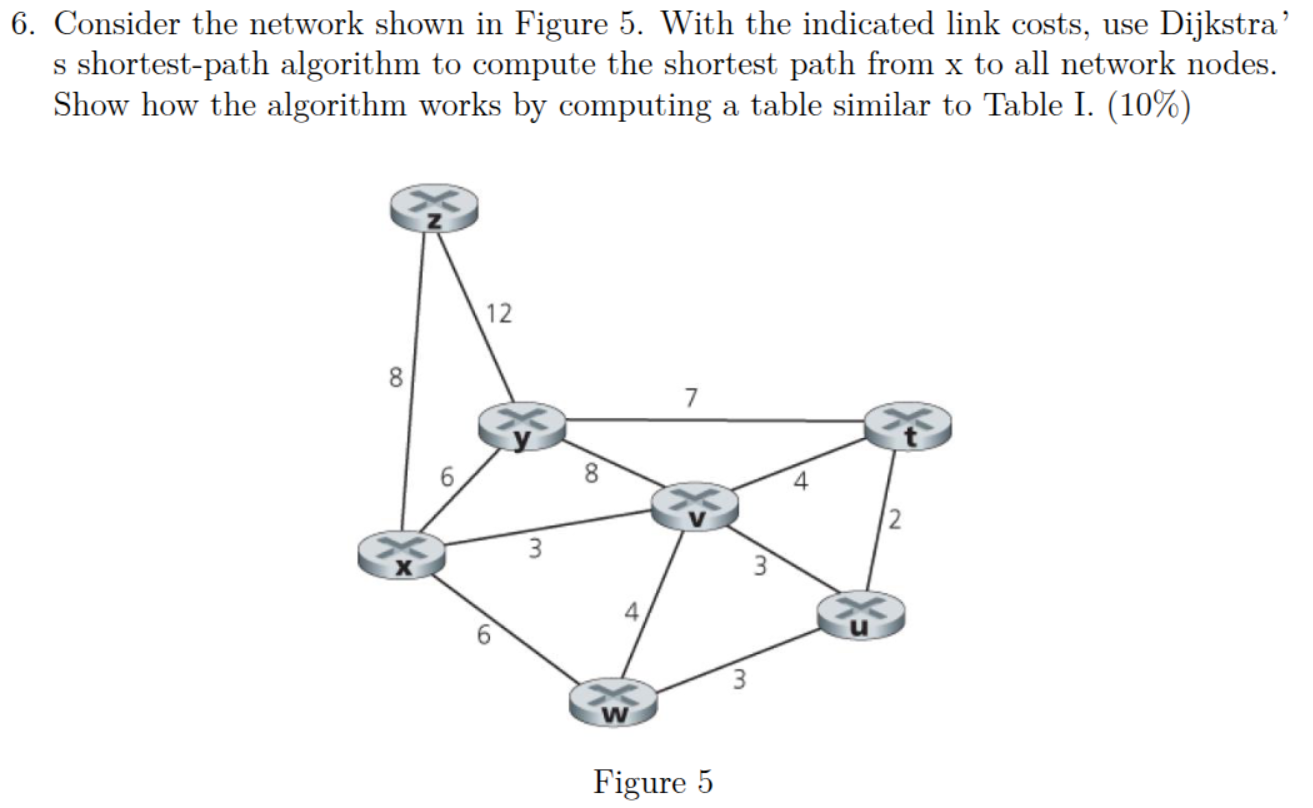
\includegraphics[width=0.8\textwidth]{src/dijkstra-example.png}
        \end{center}
    \end{frame}


    \scriptsize
    \begin{frame}[fragile]
        \frametitle{Code for Dijkstra's Algorithm}
        \begin{minted}[
            linenos,                      % 開啟行號
            frame=lines,                  % 上下框線
            framesep=5pt,                 % 程式碼與邊框距離
            numbersep=8pt,                % 行號與程式碼距離
            fontsize=\scriptsize,        % 可視需求調整字體大小
            breaklines,                  % 長行自動換行(建議)
            tabsize=4,                   % tab 寬度
            rulecolor=\color{black},     % 框線顏色
            xleftmargin=1.5em            % 讓行號有空間顯示 
        ]{cpp}
            struct edge{
                int v, w;
            };
            vector<edge> e[N];
            int dis[N], vis[N];
            void dijkstra(int n, int s){
                fill(dis, dis+N, inf);
                dis[s]=0;
                for(int i=1;i<=n;++i){
                    int u=0, min_dis=inf;
                    for(int j=1;j<=n;++j)
                        if(!vis[j] and dis[j]<min_dis)
                            u=j, min_dis=dis[j];
                    vis[u]=1;
                    for(auto ed:e[u]){
                        int v=ed.v, w=ed.w;
                        if(dis[v]>dis[u]+w)dis[v]=dis[u]+w;
                    }
                }
            }
        \end{minted}
    \end{frame}
    \begin{frame}
        What is the time complexity of the code above?

    \end{frame}
    \begin{frame}
        What is the time complexity of the code above?
        \begin{block}{Answer}
            We use double loop to find the minimum distance node,
            so the time complexity is $O(n^2)$.
        \end{block}
        If we use a priority queue to store the nodes,
        the time complexity can be reduced to $O((n+m)\log n)$,
    \end{frame}
    \begin{frame}
        \frametitle{Practice}
        \begin{itemize}
            \item \href{https://cses.fi/problemset/task/1671}{CSES 1671 - Pure Dijkstra}
        \end{itemize}
    \end{frame}
    \begin{frame}
        \frametitle{Summary}
        Dijkstra's algorithm ...
        \begin{itemize}
            \item is an $O((n+m)\log n)$, greedy algorithm.
            \item can help us find the minimum distance from \textbf{a source node} to all other nodes.
            \item can't handle negative weights.
        \end{itemize}
    \end{frame}

    % Bellman-Ford Algorithm
    \begin{frame}
        \frametitle{Bellman-Ford Algorithm}
        If there are negative weights in the graph, the Dijkstra's algorithm may not work correctly.
        In this case, we can use the Bellman-Ford algorithm, 
        a dynamic programming algorithm based on the principle of relaxation.

      
        The following steps outline the algorithm:
        \begin{enumerate}
            \item Initialize the distance to the source node as 0 and all other nodes as infinity.
            \item \textbf{Relax} all edges repeatedly for $n-1$ iterations, where $n$ is the number of nodes.
            \item Check for negative weight cycles by relaxing all edges one more time.
        \end{enumerate}
        \vspace{0.5cm}
        TL;DR:The Bellman-Ford algorithm can handle graphs with negative weights and is useful for detecting negative weight cycles.
    \end{frame}

    \begin{frame}
        \frametitle{Relaxation}
        Define \texttt{dis(u, v)} as the current shortest distance from node \texttt{u} to node \texttt{v}, 
        and \texttt{w(u, v)} as the weight of the edge from \texttt{u} to \texttt{v}. 

        The relaxation step can be defined as:
        
        \begin{equation*}
            \texttt{dis(u, v) = min(dis(u, v), dis(u)+w(u, v))}
        \end{equation*}
    \end{frame}
    
    %negative cycle
    \begin{frame}
        \frametitle{Negative Cycle}
        \begin{center}
            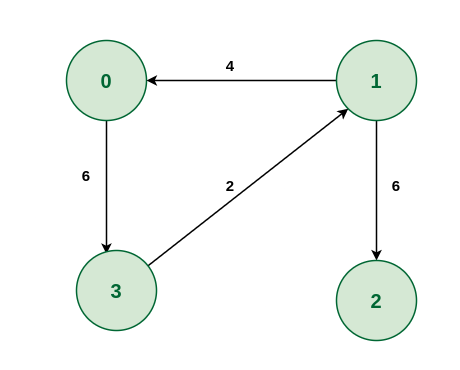
\includegraphics[width=0.6\textwidth]{src/negative-cycle.png}
        \end{center}
    \end{frame}

    \begin{frame}[fragile]
        \frametitle{Code for Bellman-Ford Algorithm-Initialize}
        \begin{minted}[
            linenos,                      % 開啟行號
            frame=lines,                  % 上下框線
            framesep=5pt,                 % 程式碼與邊框距離
            numbersep=8pt,                % 行號與程式碼距離
            fontsize=\scriptsize,        % 可視需求調整字體大小
            breaklines,                  % 長行自動換行(建議)
            tabsize=4,                   % tab 寬度
            rulecolor=\color{black},     % 框線顏色
            xleftmargin=1.5em            % 讓行號有空間顯示 
        ]{cpp}
        struct edge{
            int u, v, w;
        };
        vector<edge> e;
        int dis[N];
        \end{minted}
        
    \end{frame}

    \begin{frame}[fragile]
        \frametitle{Code for Bellman-Ford Algorithm-Function}
        \begin{minted}[
            linenos,                      % 開啟行號
            frame=lines,                  % 上下框線
            framesep=5pt,                 % 程式碼與邊框距離
            numbersep=8pt,                % 行號與程式碼距離
            fontsize=\scriptsize,        % 可視需求調整字體大小
            breaklines,                  % 長行自動換行(建議)
            tabsize=4,                   % tab 寬度
            rulecolor=\color{black},     % 框線顏色
            xleftmargin=1.5em            % 讓行號有空間顯示 
        ]{cpp}
        bool bellman_ford(int n, int s){
            fill(dis, dis+N, inf);
            dis[s]=0;
            bool relax=0;
            for(int i=1;i<=n;++i){
                relax=0;
                for(auto ed:e){
                    int u=ed.u, v=ed.v, w=ed.w;
                    if(dis[u]==inf)continue;
                    if(dis[v]>dis[u]+w){
                        dis[v]=dis[u]+w;
                        relax=1;
                    }
                }
                if(!relax)break;
            }
            return relax;
        }
        \end{minted}
        
    \end{frame}

    \begin{frame}
        What is the time complexity of the code above?

    \end{frame}
    \begin{frame}
        What is the time complexity of the code above?
        \begin{block}{Answer}
            We use double loop to find the minimum distance node,
            so the time complexity is $O(nm)$, where $n$ is the number of nodes and $m$ is the number of edges.
        \end{block}
        
    \end{frame}
    \begin{frame}
        \frametitle{Practice}
        \begin{itemize}
            \item \href{https://cses.fi/problemset/task/1672}{CSES 1672 - Pure Bellman-Ford}
            \item \href{https://cses.fi/problemset/task/1673}{CSES 1673 - Change the relax function}
        \end{itemize}
    \end{frame}
    \begin{frame}
        \frametitle{Summary}
        Bellman-Ford algorithm ...
        \begin{itemize}
            \item is an $O(nm)$, dynamic programming algorithm.
            \item can help us find the minimum distance from \textbf{a source node} to all other nodes.
            \item can handle negative weights.
        \end{itemize}
        If the graph doesn't contain any negative weights, Dijkstra's algorithm is a better choice.
    \end{frame}

    % Floyd-Warshall Algorithm
    \begin{frame}
        \frametitle{Floyd-Warshall Algorithm}
        To find the shortest path between all pairs of nodes in a graph,
        we can use the Floyd-Warshall algorithm, which is a dynamic programming algorithm.

      
        The following steps outline the algorithm:
        \begin{enumerate}
            \item Initialize a distance matrix with the weights of the edges.
            \item Iterate through all pairs of nodes and update the distance matrix by 
            considering each node as an intermediate node.
            \item If the distance from node \texttt{u} to node \texttt{v} through node 
            \texttt{k} is shorter than the current distance, update the distance.
            \item Repeat until all pairs of nodes have been considered.
        \end{enumerate}
        \vspace{0.5cm}
    \end{frame}


    \begin{frame}[fragile]
        \frametitle{Code for Floyd-Warshall Algorithm}
        \begin{minted}[
            linenos,                      % 開啟行號
            frame=lines,                  % 上下框線
            framesep=5pt,                 % 程式碼與邊框距離
            numbersep=8pt,                % 行號與程式碼距離
            fontsize=\scriptsize,        % 可視需求調整字體大小
            breaklines,                  % 長行自動換行(建議)
            tabsize=4,                   % tab 寬度
            rulecolor=\color{black},     % 框線顏色
            xleftmargin=1.5em            % 讓行號有空間顯示 
        ]{cpp}
        int mp[1005][1005][1005];
        int n,m;

        inline void warshall(){
            for(int k=0;k<n;++k)
            for(int i=0;i<n;++i)
            for(int j=0;j<n;++j)
                mp[k][i][j]=min(mp[k-1][i][j],mp[k-1][i][k]+mp[k-1][k][j]);
        }
        \end{minted}
    \end{frame}
    \begin{frame}[fragile]
        We found that k can be neglected in the code above.
        \frametitle{Code for Floyd-Warshall algorithm}
        \begin{minted}[
            linenos,                      % 開啟行號
            frame=lines,                  % 上下框線
            framesep=5pt,                 % 程式碼與邊框距離
            numbersep=8pt,                % 行號與程式碼距離
            fontsize=\scriptsize,        % 可視需求調整字體大小
            breaklines,                  % 長行自動換行(建議)
            tabsize=4,                   % tab 寬度
            rulecolor=\color{black},     % 框線顏色
            xleftmargin=1.5em            % 讓行號有空間顯示 
        ]{cpp}
        int mp[1005][1005];
        int n,m;

        inline void warshall(){
            for(int k=0;k<n;++k)
            for(int i=0;i<n;++i)
            for(int j=0;j<n;++j)
                mp[i][j]=min(mp[i][j],mp[i][k]+mp[k][j]);
        }
        \end{minted}
    \end{frame}

    \begin{frame}
        What is the time complexity of the code above?

    \end{frame}
    \begin{frame}
        What is the time complexity of the code above?
        \begin{block}{Answer}
            We use triple loop to find the minimum distance node,
            so the time complexity is $O(n^3)$, where $n$ is the number of nodes.
        \end{block}
    \end{frame}

    \begin{frame}
        \frametitle{Summary}
        \begin{itemize}
            \item Floyd-Warshall algorithm is simple but slow, it also occupy lots of memory.

            \item We can use Dijkstra or Bellman-Ford algorithm to replace it in most cases.

            \item But if the graph is hugely dense,
            the Floyd-Warshall algorithm can be more efficient than Dijkstra or Bellman-Ford
            because it can find the shortest path between all pairs of nodes in one go.
            \item Think about it, how to detect negative cycles in the graph with Floyd-Warshall algorithm?
        \end{itemize}
    \end{frame}
        \begin{frame}
        \frametitle{Practice}
        \begin{itemize}
            \item \href{https://cses.fi/problemset/task/1197}{CSES 1197}
            \item (optional)\href{https://www.luogu.com.cn/problem/P3403}{Luogu P3403 - implicit graph}
            \item (optional)\href{https://codeforces.com/problemset/problem/1540/A}{CF 1540A - Construct a Graph}
        \end{itemize}
    \end{frame}
    \begin{frame}
        \frametitle{More about it}
        \begin{itemize}
            \item kth shortest path problem
            \item Johnson's algorithm
            \item A* algorithm
            \item implicit graph(i.e. \href{https://leetcode.com/problems/water-and-jug-problem/description/}{measuring jugs problem})
        \end{itemize}
    \end{frame}
\end{document}